\chapter{牛人简历}{Resumes of Supermans}
\label{cha:ResumesOfSupermans}
\section{Knuth 教授简历}{Resume of Pro. Knuth}

1938 年 12 月 7 日, Donald E. Knuth 出生于美国威斯康星州密尔沃基市. 其父是个中学教
师, 经常在星期天到教堂演奏管风琴, 小 Knuth 耳濡目染, 日后也成为教师, 业余爱好也是
弹管风琴.

\begin{figure}
  \centering
  \begin{minipage}[t]{0.3\textwidth}
    \centering
    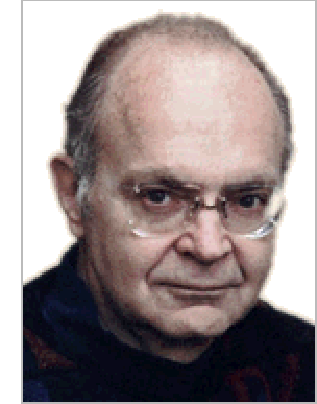
\includegraphics[width=3cm]{KnuthPhoto.pdf}
    \caption{Knuth 教授头像}{The head portrait of Pro. Knuth}
  \end{minipage}
  \hspace{1cm}
  \begin{minipage}[t]{0.3\textwidth}
    \centering
    \includegraphics[width=3.8cm]{knuthPhotoCartoon.pdf}
    \caption{Knuth 教授卡通头像}{The cartoon portrait of Pro. Knuth}
  \end{minipage}
\end{figure}


1956 年进入俄亥俄州克利夫兰的凯斯理工学院 (现并入凯斯西储大学), 学习物理.

1957 年大学一年级暑假在学校打工, 接触到当时很先进的 IBM650 计算机, 产生浓厚兴趣.

1958 年改学数学, 并从此与计算机结缘.

1960 年毕业, 因为成绩过于出色, 校方打破惯例, Knuth 被同时授予学士和硕士学位. 随后
进入加州理工学院数学系.

1960 -- 1968 年, 兼任 Burroughs 公司顾问.

1961 年结婚, 夫人小他一岁. 现有一儿一女.

1963 年取得博士学位, 并留校任助理教授.

1964 -- 1967年, 兼任美国计算机协会刊物《程序设计语言》编辑.

1966 年升为副教授.

1968 年任教于斯坦福大学计算机科学系, 正教授. 同年, 开始撰写著名的《计算机程序设计
艺术》一书.

1968 年《计算机程序设计艺术》第一卷《基本算法》出版.
1969 年, 第二卷《半数字化算法》出版.
1971 年获首届美国计算机协会格蕾丝 $\cdot$ 赫柏奖.
1973 年, 第三卷《排序与搜索》出版. 同年还出版了第一卷的第二版. 有人曾说, 看了这部
书后, 再谈起编程序都会变得谦虚谨慎. 比尔 $\cdot$ 盖茨曾说:``如果你能读懂整套书的
话,请给我发一份你的简历."同年, 当选为美国科学艺术学院院士. 截至到 1973 年的第一卷
第二版, 采用都是的活字排版印刷, 这需要经验丰富的活字排版工人.

1974 年, 因在算法分析和编程语言设计方面的突出贡献, 荣获美国计算机协会图灵奖, 是历
史上最年轻的获奖者. 图灵奖被称为计算机界的诺贝尔奖. 《计算机程序设计艺术》一书与
牛顿的《自然哲学的数学原理》等书一起, 被评为``世界历史上最伟大的十种科学著作"之一.

1975 年当选为美国国家科学院院士.

1976 年出版第二卷第二版时采用了计算机排版技术. 但是, 当时的计算机排版与活字排版效
果相差甚远, 而且前后两卷的字体、版式和文本格式等都不一致. 非常失望的 Knuth 暂停了
第二卷第二版的出版, 决心自己设计一个比活字排版更加优美和适用的排版软件, 这就是后来
的 \TeX.

1977 年 5 月开始构造后来被称为 \TeX{} 的文字处理系统, 他研究了古今的排版技术, 把其
中最优越的部分引入 \TeX{} 中, 连 \TeX{} 中的字体 (METAFONT) 全部都是他自行设计的.
同年, 访问中国三周, 行前姚储枫给他起了个中文名字: 高德纳. (姚储枫, 姚期智的夫人,
夫妇都是著名计算机科学家, 2000 年姚期智获图灵奖.)

1978 年应邀在美国数学学会年会上作报告, 题为``数学排版 --- \TeX{} 与 METAFONT",引起
数学界关注.

1979 年, Knuth 教授的著作《\TeX{} 与 METAFONT: 排版的新趋势》, 由数字设备公司和美
国数学学会联合出版. 同年, 荣获美国总统卡特授予的科学金奖.

1980 年获国际电子电气工程师协会计算机学会麦可道尔奖. 同年, 成为英国计算机学会会员.

1981 年当选为美国工程院院士.

1982 年使用自己设计的 \TeX{} 软件和字体, Knuth 如愿出版了《计算机程序设计艺术》的第
二卷第二版. 之后, Knuth 还不遗余力地改进 \TeX, 并在 \TeX{} 的稳定性上下了很大功夫.
在基本式样没有改变的情况下, \TeX{} 第 3 版又追加了很多功能. 9 月, 公布了 DVI 驱动
程序. 同年, 成为国际电子电气工程师协会荣誉会员, 并获计算机先锋奖.

1984 年, 艾迪生---韦斯利公司出版 Knuth 教授的《The TeXbook》, 该书成为最权威的 \TeX{}
参考书.

1985 年, 将 \TeX{} 的默认字体由美国现代改为计算机现代.

1986 年荣获美国数学学会的斯蒂尔奖.

1987 年获纽约科学研究会奖.

1988 年获富兰克林奖.

1989 年, 因其对软件理论的贡献获 J.D. Warnier 奖.

1990 年, 斯坦福大学授予他计算机科学艺术教授的称号.

1991 年, 《3:16 圣经文本阐释》一书出版, 他试图用分层随机抽样的方法对圣经进行分析.

1992 年退休, 但还是斯坦福大学和牛津大学的客座教授. 他这么早退休的原因, 就是因为研究
开发 \TeX{} 系统延误了编写出版《计算机程序设计技巧》这部书, 他估计还要花 20 年来完
成. 目前此书前三卷已出版, 预计要出到第七卷.

1993 年宣布不再对 \TeX{} 和 METAFONT 进行更新.

1994 年获瑞典皇家科学院克努特奖.

1995 年获国际电子电气工程师协会的纽曼奖和以色列的科学与艺术哈维奖.

1996 年 11 月, 由于发明先进的排版技术荣获京都先进技术奖 (日本最高终身成就奖, 奖金
约 46 万美元, 被称为日本的诺贝尔奖).

1997 年对《计算机程序设计技巧》前三卷作了修订.

2001 年国际天文学联合会把两年前发现的第 21656 号小行星命名为``Knuth".

2003 年荣获马其顿大学荣誉博士, 同年当选英国皇家学会的外籍院士.

2004 年《计算机程序设计技巧》前三卷再版发行.

\begin{figure}
  \centering
  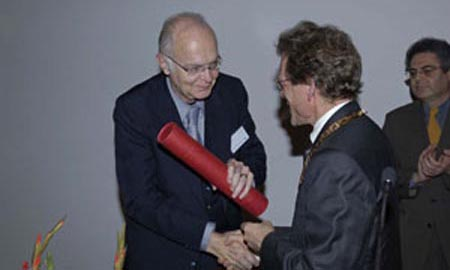
\includegraphics[width=9cm]{Knuth2005.jpg}\\
\end{figure}

2005 年 11 月, 从瑞士联邦苏黎士高等理工学院院长手中接过荣誉博士证书.

现在, 正在编写《计算机程序设计技巧》其余几卷.
 
他的所有著作都有个奇特``附加效应", 那就是任何人发现书中的错误, 不论是技术上的或是
排版上的还是历史上的错误, 都可以向他指出, 并可领取 2.56 美元! 可见其人幽默诙谐而且
能够闻过则喜.

\begin{figure}
  \centering
  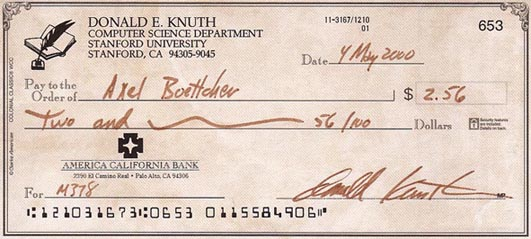
\includegraphics[width=10cm]{KnuthCheck.jpg}\\
  \caption{Knuth 教授的支票}{The check of Pro. Knuth}
\end{figure}


为什么是 2.56 美元? Knuth 教授的答案是:``256 pennies is one hexadecimal dollar."
 
从 1981 年夏至 1996 年 7 月 1 日, Knuth 教授给指出错误的人回信 250 多封, 其中一半
以上装有奖励支票. 从奖励支票清单来看, 有一位名叫 Axel B\"{o}ttcher  的人, 曾先后 5
次得到两块五毛六的支票, 3 次得到五块一毛二的支票, 真可谓牛人背后有牛人.
 
受麦粒与棋盘的故事影响, Knuth 教授宣布, 每发现一个 \TeX{} 程序或 METAFONT 程序中的
错误, 奖励从 2.56 美元开始, 每年翻倍, 最高为 327.68 美元. 1995 年有两人领取了这项
奖金, 此后至今, 还无人能够认领!
 
有网友戏说, 什么是聪明: 在 Knuth 的书中找到错误; 什么是愚蠢: 去兑现那张两块五毛六的
支票.
 
Knuth 教授是法国、挪威和德国科学院的外籍院士; 还是牛津大学、巴黎大学、斯德哥尔摩皇
家理工学院、奥斯陆大学、安特卫普大学、圣彼得堡大学和马其顿大学等十几所大学的荣誉博士.

Knuth 教授带过 28 个研究生, 拥有 5 项专利, 出版 25 部著作, 发表 160 篇论文; 他的著
作已有 6 种文字译本, 发行量超过一百万册. 英文版的《计算机程序设计艺术》一书已再版
11 次, 该书前三卷中文版于 1978 年至 1992 年陆续出版, 由苏运霖教授翻译, 他曾在 1977
年与来访的 Knuth 教授在北京座谈.

Knuth 教授爱好音乐, 年轻时曾考虑报考音乐专业. 在他的书房中放了一个特别定制的 84 管
的管风琴. 他还会吹萨克斯管和大号.
            
\TeX{} 是二十世纪排版技术方面最重大的发明, 历经 20 年的岁月, \TeX{} 在基本没有改动
的情况下被世界各地各种语言的人们广泛使用, \TeX{} 的优美排版效果令使用者爱不释手.
现在, 世界上很多国家都有 \TeX{} 用户组织, \TeX{} 不断地被推广和扩展.

Knuth 教授因在 \TeX{} 及计算机编程方面的巨大贡献和他大量创造性的影响深远的著作而享
誉全球.

Donald E. Knuth 这个名字将和 \TeX{} 一起被载入世界科学史册.

\section{Lamport 博士简历}{Resume of Pro.Lamport}

\begin{figure}
  \centering
  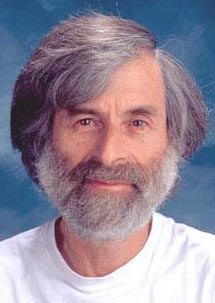
\includegraphics[width=4cm]{LeslieLamport.jpg}\\
  \caption{Lamport 教授的头像}{The head portrait of Pro. Lamport}
\end{figure}

1941 年 Leslie Lamport 生于纽约.

1960 年毕业于麻省理工学院数学专业.

1963 年获得布兰迪斯大学数学硕士学位.

1965 -- 1969 年任教于马尔波罗学院.

1970 -- 1972 年, 麻省计算机协会系统设计员.

1972 年获得布兰迪斯大学数学博士学位.

1972 -- 1977 年, 麻省计算机协会研究员.

1977 -- 1985 年, SRI 公司计算机科学实验室任究员.

1982 年与另两人共同发表论文``拜占廷将军问题", 既允许军中可能有叛徒, 又要保证战争胜
利, 引申到计算机领域, 成为一种容错理论.

1984 年前后, 使用 Knuth 教授发明的 Plain \TeX{} 排版软件撰写一些并行计算方面的论文,
感到还是不太方便, 于是编写了便于自己使用的宏包套件, 并命名为 \LaTeX. 其主要改进是将
版面设计与文稿内容分开处理, 只要使用者选择了一种文件类别, \LaTeX{} 自动将整本书或整
篇文章的结构和标题就按照这种文件类別典型样式来设置, 作者只要专注文章的內容就可以了.
起初 \LaTeX{} 在计算机科学家之间流传, 大家觉得 \LaTeX{} 比 Plain \TeX{} 使用更方便,
就经常通过各种渠道向他索取.

1984 年发表论文``分布系统中的时间、时钟和事件排序".

1985 -- 2001 年, 在数字设备公司以及康柏系统研究中心作研究工作. (1998年, 康柏计算机
公司收购了数字设备公司. 2002 年惠普公司完成收购康柏公司之后, 数字设备公司的剩余部分
并入了惠普公司. )

1985 年, 花两个月时间将 \LaTeX{} 源代码整理出来, 并编写出版了一本 \LaTeX{} 使用手册
《\LaTeX: 一种文稿排版系统》, 当时流行的 \LaTeX{} 版本为 2.09.

1989 年 8 月 21 日, 在斯坦福大学 \TeX{} 用户组织会议上, 同意将 \LaTeX{} 的维护和开
发工作交给 \LaTeX{}3 小组.

1994 年, 与 \LaTeX{}3 小组对 \LaTeX{} 作了一次重大改进, 版本命名为 \LaTeX{}2$\varepsilon$,
并出版 \LaTeX{} 使用手册第二版.

\begin{figure}
  \centering
  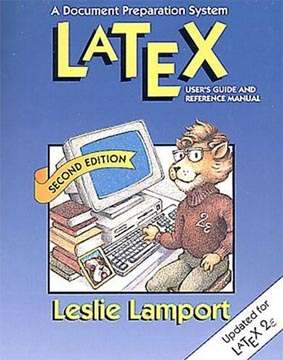
\includegraphics[width=6cm]{LaTeXADocumentPreparationSystem.jpg}\\
  \caption{\LaTeX: 一种文稿排版系统封面}{\LaTeX: A document preparation system}
\end{figure}


2001 年进入位于加利福尼亚的微软研究院, 任高级研究员, 从事分布式计算机系统理论研究.

2003 年获法国雷恩大学荣誉博士.

\begin{figure}
  \centering
  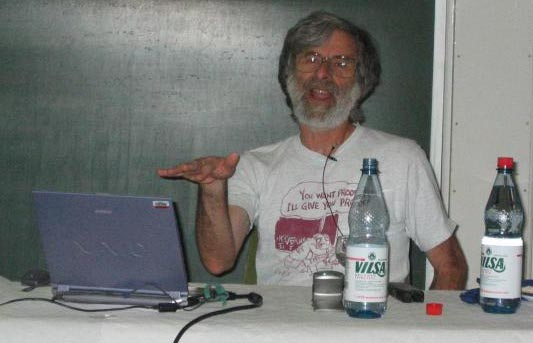
\includegraphics[width=8cm]{LamportYouWantProof.jpg}\\
  \caption{德国基尔大学作学术报告}{Lecture in Christian-Albrechts-Universit\"{a}t zu Kiel}
\end{figure}

2004 年, 由于在计算机信息处理方面的突出贡献, 获得皮奥尔奖. 同年获瑞士洛桑联邦工业
大学荣誉博士.

截至 2006 年, 已发表论文 160 篇.
